%\documentclass[12pt]{scrreprt}
\documentclass[12pt]{report} 

% language may be romanian or english (default is english)
% type may be bachelor or master (default is bachelor)
\usepackage[language=romanian, type=bachelor]{style}

%\geometry{a4paper,top=2.5cm,left=3cm,right=2.5cm,bottom=2.5cm}
%in style
%controlling the appearance of your headers and footers
\usepackage{fancyhdr}
\pagestyle{fancy}
\lhead{}
\chead{}
\renewcommand{\headrulewidth}{0.2pt}
\renewcommand{\footrulewidth}{0.2pt}

\begin{document}

\specialization{INFORMATICA}	
\title{SISTEM PENTRU RECOMANDARE DE FILME}					   
\author{RADU DRAGOS STEFAN}											
\supervisor{[Grad, titlu si nume coordonator]}				
				
\maketitle


\newpage
\thispagestyle{empty}
\mbox{}
\newpage
\pagenumbering{roman} 

\cleardoublepage
ABSTRACT
\vspace{0.5cm}	
\hrule
\vspace{0.5cm}	
%\cleardoublepage

Abstract: un rezumat \^{i}n limba englez\u{a} cu prezentarea, pe scurt, a con\c{t}inutului pe capitole, pun\^{a}nd accent pe contribu\c{t}iile proprii \c{s}i originalitate



\tableofcontents


\newpage
\pagenumbering{arabic}

%\chapter{Introducere}

%\chapter*{Introducere}
\label{intro}

\par Introducere: obiectivele lucrarii si descrierea succinta a capitolelor, prezentarea temei, prezentarea contributiei proprii, respectiv a rezultatelor originale si mentionarea (daca este cazul) a sesiunii de comunicari unde a fost prezentata sau a revistei unde a fost publicata.
%\addcontentsline{toc}{chapter}{Introducere}
%\addcontentsline{toc}{chapter}{Introduction}

\pagenumbering{arabic}
\input{chapters/chapter1.0}
\chapter{Cadru de lucru }
\section{Problema propusa}
\label{sec:ch3sec1}

\par Utilizatorul doreste ca pentru filmele pe care el le-a vizionat sau pe care le considera importante el sa poata primi recomandari. Algoritum calculeaza o matrice de scoruri in funtie de similaritatea cosinus si de rating ul filmelor si va returna utilizatorului filmele cu  cele mai bune scoruri pentru un anumit film sau pentru lista de filme.

\section{Solutie}
\par Solutia e compusa din mai multe parti. In primul rand, e nevoie de o baza de date populate cu filme care sa fie bine descrise astfel algorituml sa poata recomanda cele mai bune filme. Dupa o vreme dupa ce aplicatia va fi folosita aceasta va da un randament si mai bun din cauza ca utilizatorii vor intoduce rating uri. Urmatorul pas si poate unul din cele mai dificile este dezvoltarea algoritmului care va face recomandarile de filme. Ultima parte va consta din crearea unei interfete , un site web deoarece poate fi accesat si de pe telefon dar si de pe un calculator, in care utilizatorul sa isi poata intretine propia lui lista de flme. Pe baza acestor filme se vor face recomandari cu ajutorul algoritumului.
\chapter{Capitolul 1: Algoritmul de recomandare }
\label{chap:ch1}

\section{Prelucrarea datelor}
\label{sec:ch3sec1}
\par Un prim pas in algoritmul de recomandare de filme este de a prelucra datele pentru a obtine cele mai bune valori in calculul final al scorului. Dupa ce avem toate datele un prim pas este sa inlocuim datele nule cu caracterul spatiu pentru a nu conta in calculul final. Apoi un pas destul de important in procesarea datelor este sa eliminam cuvintele de legatura ca de exmplu:  ‘an’, ‘be’, ‘some’, etc.  Cel mai important camp din care trebuie scoase aceste cuvinte este descrierea deoarece la final se vor crea vectori din cuvintele pe care le avem in datele noastre, iar cuvintele de legatura nu sunt deloc importante in calculul final noi avand nevoie doar de cuvintele estentiale. Ultimul lucru care trebuie facut in procesarea datelor este de a scoate separatorii de cuvinde, in datele noastre fiind doar virgula, din colonele:gen, actori, scriitori, directori si descriere. 

\section{Sacul de cuvinte si transformrea cuvintelor in vectori }
\par Urmatorul pas in algorituml de recomandare de filme este de a creaa cea ce se numeste “Bag of words”. Modelul “Bag of words” este o reprezentare pentru procesarea limbajului natural și regăsirea informațiilor care simplifică lucrurile (IR). Un text (cum ar fi o propoziție sau un document) este reprezentat în această paradigmă ca un sac (multiset) al cuvintelor sale, care ignoră sintaxa și chiar ordinea cuvintelor, păstrând în același timp multiplicitatea. Viziunea computerizată a utilizat, de asemenea, conceptul de sac de cuvinte. Pentru a creea sacul de cuvinte se lipesc toate toate datele de care avem nevoie in calculul scorului final: descrierea fara cuvinte de legatura,gen, actori, scriitori, directori si descriere, intr-un singur camp pe care il numin “bag” aceasta operatie facandu-se pentru fiecare film, deci fiecare film va avea propiul bag. Urmatorul pas este de a pune toate bag-urile la un loc si de a scoate duplicatele la urma ramanand cu n cuvinte care apar in datele din toate filmele.  Pe baza acestor cuvinte se va creea pentru fiecare film cate un vector de dimensiune n fiecare pozitie reprezentand frecventa cuvantului din filmul curent. Ca exeplu pentru explicatia de mai sus luam trei propozitii: 
		\begin{figure}[htbp]
			\centerline{
\includegraphics[width=16cm, height=4cm]{figures/cele 2 poze.png}}
			\caption{Propozitii pentru exemplu}
			\label{fig}
		\end{figure}
\par Dupa ce scoatem cuvintele de legatura:lui, ii, sa, se, propozitiile prima propozitie va arata Daniel, place, uite, filme , iar a doua Marius place uite fotbal. Dupa ce se lipesc cele doua propozitii campul cuvintelor va fi: Daniel, place, uite, filme, Marius, fotbal. Apoi vectori care se vor creea pentru cele doua propozitii vor arata in felul urmator: 

		\begin{figure}[htbp]
			\centerline{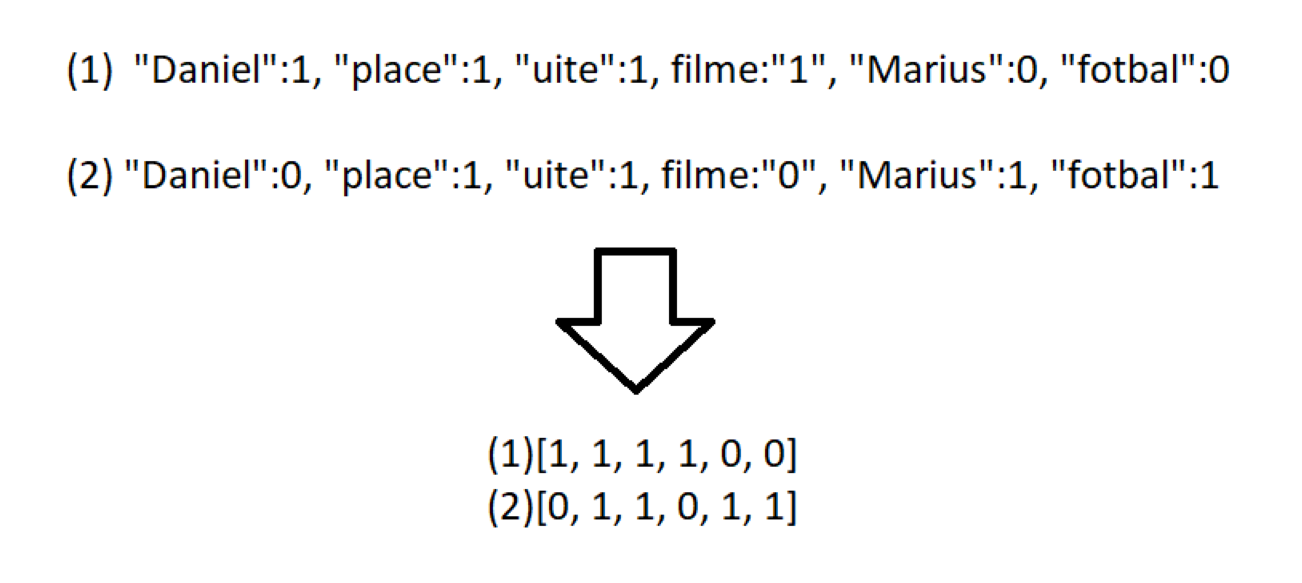
\includegraphics[width=16cm, height=9cm]{figures/rezultat vectori.png}}
			\caption{Propozitii pentru exemplu}
			\label{fig}
		\end{figure}

\section{Similaritatea cosinus }
\par Metrica de similaritate cosinus este utilizată pentru a determina cât de asemănătoare sunt documentele, indiferent de mărimea lor. Aceasta estimează matematic cosinusul unghiului format de doi vectori proiectați într-un spațiu multidimensional. Similaritatea cosinusului este utilă deoarece, chiar dacă două documente comparabile sunt separate de o distanță euclidiană mare (din cauza dimensiunii documentelor), este probabil ca acestea să fie similare. Pentru acest model, se foloseste similaritatea cosinusului pentru a defini "similitudinea" dintre filme.Motivul pentru care nu se folosește doar distanța dintre vectori ca scor de similaritate, chiar dacă ar putea părea rezonabil, lungimile vectorilor pot afecta distanța euclidiană, dar nu și distanța cosinus (1 - cos(unghi)). Deoarece lungimile a doi vectori definesc dimensiunea acestora (de exemplu, cantitatea de date), dar unghiul definește mai bine caracteristicile lor în lipsa unor cuvinte mai bune. Prin urmare, distanța unghiulară este mai potrivită pentru a defini similitudinea lor.
		\begin{figure}[htbp]
			\centerline{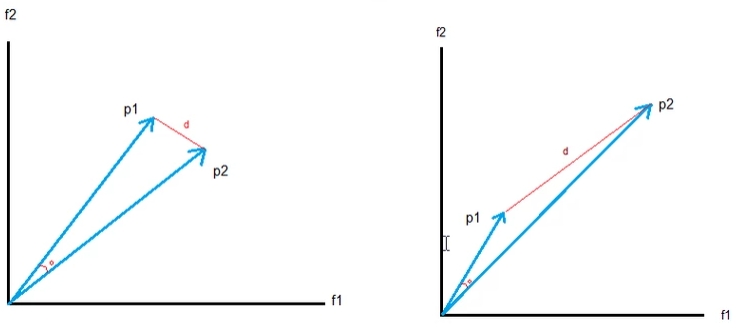
\includegraphics[width=12cm, height=5cm]{figures/grafic distanta.png}}
			\caption{Distanca euclidiana vs. distanta ungiulara}
			\label{fig}
		\end{figure}
\par După cum se poate  vedea, distanța euclidiană devine mult mai mare pe al doilea grafic, chiar dacă unghiul este destul de mic.

\section{Calcularea scorului final}
\par Dupa ce se calculeaza o matrice in care perechea (i,j) reprezinta similaritatea cosinus dintre doua filme se calculeaza inca o matrice care va reprezenta scorul final. Similaritatea cosinus va fi imbunatatita in functie de cat de apreciat este un film, astfel zece procente din scorul final le va reprezenta media dintre suma voturilor si numarul de votanti. La final se vor lua cele mai mari n scoruri , n reprezentand numarul de filme pe care vrem sa le recomandam, exceptandul pe primul deoarece cel mai bun scor il va avea filmul insusi.
\chapter{Titlul capitolului}
\label{chap:ch1}





\chapter{Capitolul 3: Tehnologiile de pe Back-end}
\label{chap:ch3}

\section{Node Js}
\label{sec:ch3sec1}

\par Node js este un ecosistem de JavaScript , open-source , cross-platform si care este bazat pe motorul V8 de la Chrome acesta executand cod JavaScript in afara unui browser web. Node.js permite programatorilor să folosească JavaScript pentru a crea instrumente in  linia de comandă și scripturi pentru servere  cu ajutorul carora se  generează conținutul dinamic pe paginiile web înainte ca pagina să fie transmisă către browserul utilizatorului.
\par JavaScript a fost creat ca un limbaj de programare care se baza pe browser si care avea un singur fir de execuție. A fi single-threaded înseamnă că, în același proces, se execută un singur set de instrucțiuni la un moment dat (în acest caz, browserul, sau doar fila curentă în browserele moderne). Datorita acestui lucru s-au ușurat lucrurile pentru dezvoltatorii care folosesc acest limbaj. JavaScript a fost inițial un limbaj util numai pentru adăugarea unor interacțiuni la paginile web, validări de formulare și așa mai departe - nimic care să nu necesite complexitatea multithreading-ului.
Cum funcționează in spate este destul de interesant, în comparație cu tehnicile tradiționale de servire web în care fiecare conexiune (cerere) generează un fir nou, preluând RAM de sistem și, în cele din urmă, maximizând cantitatea de RAM disponibilă, Node.js funcționează pe un singur fir, utilizând  apeluri non-blocante, permițându-i să suporte zeci de mii de conexiuni simultane ținute în bucla evenimentului
\par Cand vorbim de node js este foarte important de mentionat este suportul incorporat pentru gestionarea pachetelor utilizand NPM(node package manager), un instrument care vine în mod implicit la fiecare instalare Node.js. Modulele NPM sunt comparabile cu Ruby Gems în sensul că sunt o colecție de componente reutilizabile disponibile în mod public, care pot fi instalate cu ușurință dintr-un depozit online și includ gestionarea versiunilor și a dependențelor. Oricine poate contribui la ecosistemul de module prin publicarea propriului modul pentru a fi inclus în depozitul npm.

\section{Javascript}
\label{sec:ch3sec2}

\par Limbajul de programare JavaScript și-a petrecut cea mai mare parte a vieții în interiorul browserele web. A început ca un limbaj de scripting de bază pentru ajustarea celor mai fine aspecte ale paginilor web, dar acum a evoluat într-un limbaj sofisticat cu o gamă largă de aplicații și biblioteci. Mulți furnizori de browsere precum Mozilla și Google au început să pompeze resurse în timpii de rulare rapid JavaScript, iar browserele au obținut motoare JavaScript mult mai rapide ca un rezultat.În 2009, a apărut Node.js. Node.js a scos V8, puternicul motor JavaScript Google Chrome, din browser și i-a permis să ruleze pe servere.În browser, dezvoltatorii nu au avut de ales decât să aleagă JavaScript. Dezvoltatorii pot folosi acum JavaScript în loc de Ruby, Python, Java și alte limbaje pentru a crea aplicații pe partea serverului. Deși JavaScript poate să nu fie cel mai bun limbaj pentru toată lumea, Node.js oferă o mulțime de avantaje. Pentru început, motorul JavaScript V8 este rapid, iar Node.js suportă codarea asincronă, care accelerează codul evitând în același timp problemele de multithreading. Dezvoltatorii nu trebuie să facă niciun fel de schimbare de context atunci când trec de la client și Server. 

\section{MySQL}
\label{sec:ch3sec3}

\par MySQL este un sistem de gestionare a bazelor de date relaționale dezvoltat de MySQL AB din Suedia și publicat sub Licența Publică Generală GNU. Este cel mai utilizat sistem de gestionare a bazelor de date open-source în prezent și reprezintă o parte importantă a stivei LAMP (Linux, Apache, MySQL, PHP).
\par Deși este folosit foarte des împreună cu limbajelel de programare JAVA, PHP, cu MySQL pot construi aplicații în orice limbaj major. Există multe scheme API disponibile pentru MySQL ce permit scrierea aplicațiilor în numeroase limbaje de programare pentru accesarea bazelor de date MySQL. O interfață de tip ODBC denumită MyODBC permite altor limbaje de programare ce folosesc această interfaţă, să utilizeze bazele de date MySQL cum ar fi ASP sau Visual Basic  (Molnar). 
\par Multe manuale susțin că MySQL este simplu de învățat și de utilizat în comparație cu alte programe de gestionare a bazelor de date; de exemplu, comanda exit este simplă: "exit" sau "quit". 
\par Pentru a administra bazele de date MySQL se poate folosi modul linie de comanda sau se pot descărca de pe internet diferite programe ce creează o interfață grafică: MySQL Administrator şi MySQL Query Browser. Un alt instrument de management al acestor baze de date este aplicaţia SQL Manager. 
\par MySQL este un server de baze de date care este extrem de rapid, fiabil și simplu de utilizat. A fost creat pentru a gestiona baze de date uriașe mult mai rapid decât alternativele anterioare.
\par Software-ul de baze de date MySQL este un sistem client/server care include un server MySQL cu mai multe fire și o varietate de aplicații client și biblioteci, precum și instrumente de administrare și o varietate de interfețe de programare a aplicațiilor.
 
\section{Python}
\label{sec:ch3sec4}

\par Python este un limbaj de programare dinamic semantic, de nivel înalt, orientat pe obiecte și interpretat. Structurile sale de date integrate de nivel înalt, împreună cu tastarea dinamică și legarea dinamică, îl fac ideal pentru crearea rapidă de aplicații, precum și pentru utilizarea ca limbaj de scripting sau ca punct de legătură între componentele existente. Sintaxa de bază a limbajului Python, ușor de învățat, acordă prioritate lizibilității, reducând costurile de întreținere a software-ului. Modulele și pachetele sunt suportate de Python, ceea ce facilitează modularitatea programelor și reutilizarea codului. Interpretorul Python și biblioteca standard extinsă pot fi descărcate și distribuite gratuit în formă sursă sau binară pentru toate platformele majore.
\par Python este popular în rândul programatorilor datorită productivității îmbunătățite pe care o oferă. Ciclul editare-testare-depanare este foarte rapid, deoarece nu există o fază de compilare. Depanarea scripturilor Python este simplă: o problemă de segmentare nu este niciodată cauzată de o greșeală sau de o intrare incorectă. În schimb, atunci când interpretorul găsește o greșeală, aruncă o excepție. Interpretul produce o urmă de stivă dacă aplicația nu reușește să detecteze eroarea. Se pot verifica variabilele locale și globale, se pot evalua expresii arbitrare, se pot crea puncte de întrerupere, se poate parcurge codul rând pe rând și așa mai departe cu un depanator la nivel de sursă. Depanatorul este construit în Python, demonstrând capacitățile introspective ale limbajului. Pe de altă parte, adăugarea câtorva comenzi de tastare la codul sursă este frecvent cea mai rapidă metodă de depanare a unui program: ciclul rapid editare-testare-depanare face ca această tehnică de bază să fie foarte eficientă.

\section{Flask}
\label{sec:ch3sec5}

\par Flask este un framework web scris în Python care este clasificat ca un microframe, deoarece nu necesită anumite instrumente sau biblioteci.Nu are un strat de abstractizare a bazei de date, validarea formularelor sau orice alte componente în care bibliotecile terțe preexistente oferă funcții comune. Cu toate acestea, Flask acceptă extensii care pot adăuga caracteristici ale aplicației ca și cum ar fi implementate în Flask în sine. Există extensii pentru mapere relaționale obiect, validarea formularelor, gestionarea încărcărilor, diverse tehnologii de autentificare deschise și mai multe instrumente comune legate de cadru.
\chapter{Capitolul 4: Tehnologiile de pe Front-end}
\label{chap:ch3}

\section{React}
\label{sec:ch4sec1}

\par Des considerat un JavaScript framework precum Angular sau Vue.js, React este de fapt o biblioteca de tip open source. Este folosit mai ales pentru interfate web mari, complexe dar si pentru aplicatii single-paged. Creat de Jordan Walke, un software engineer la Facebook, a fost implementat rapid in news feed-ul Facebook, in 2011. Un an mai tarziu, Instagram, aplicatia detinuta de Facebook, a implementat React si de aici incepe povestea. In ziua de azi, sute de mii (poate chiar milioane) de website-uri sunt sutinute de aceasta librarie si alte mii se nasc in fiecare zi. De fapt, de la lansarea React, am observat o crestere exploziva in utilizarea de librarii JavaScript mici ca dimensiuni, dar puternice. Utilizatorii vor sa utilizeze din ce in ce mai mult pagini web mai rapide si mai dinamice, in timp ce dezvoltatorii opteaza pentru medii moderne si flexibile fara tone de linii de cod in pachet. De aceea ReactJS este o alegere evidenta pentru multi. Ca sa explicam de ce, haideti sa recapitulam principalele motive pentru care folosim React. Desi considerat un JavaScript framework precum Angular sau Vue.js, React este de fapt o biblioteca de tip open source. Este folosit mai ales pentru interfate web mari, complexe dar si pentru aplicatii single-paged.
\par Primul lucru care face atat de multi oameni sa foloseasca ReactJS in proiectele lor este probabil simplitatea sa. React este o biblioteca JavaScript, astfel incat daca un dezvoltator este familiarizat cu functiile JS, va avea un start mai usor cu ReactJS. Cu această biblioteca, dezvoltatorii definesc interfete cu o sintaxa asemanatoare HTML numită JSX. Drept urmare, este produs cod HTML și CSS. API-ul React este foarte mic, dar puternic si tot ce trebuie safaci inainte de a incepe este sa inveti cateva functii de baza. Un pic din curba de învatare apare cand doriti sa utilizati React cu alte biblioteci JS, cum ar fi Redux, Material UI sau Enzyme. Desi nu fac parte din stiva React, astfel de biblioteci adauga functii suplimentare si va permit sa gestionati mai usor componentele React. Cele mai comune biblioteci sunt bine documentate si nu ar trebui sa creeze probleme niciunui dezvoltator.
\par React JS folosește câteva extensii numite JSX și Virtual DOM pentru a crea interfețe utilizator. Acestea permit dezvoltatorilor să le creeze pentru majoritatea platformelor și, datorită faptului că pot vedea rezultatele codului lor instantaneu, pot avea o vizualizare și o înțelegere mai bună a ceea ce fac.React JS folosește ceva numit JSX. Aceasta este o extensie a React care permite utilizarea HTML cu JavaScript și acest lucru face ca codul dvs. să fie mai versatil. React este compatibil cu majoritatea browserelor moderne, ceea ce îi ajută pe dezvoltatori să își schimbe și să testeze DOM pe diferite platforme.Virtual DOM: DOM este prescurtarea pentru Document Object Model, care este o interfață de program de aplicație (API). Permite programelor să citească conținutul oricărui site web, astfel încât să poată fi modificat în funcție de preferințele și nevoile programatorului. Orice site web care nu folosește React JS folosește HTML pentru a modifica și modifica DOM-ul său.
Datorită implementării JSX, React JS poate avea un DOM virtual, care este o copie a DOM-ului original utilizat de aplicație sau site-ul web. Principala diferență dintre DOM și DOM-ul virtual este că primul arată doar modificările după ce pagina este încărcată din nou, în timp ce acesta din urmă le arată în timp real, fără a fi nevoie să reîncărcați.

\section{TypeScript}
\label{sec:ch4sec2}

\par TypeScript a fost făcut public pentru prima dată în octombrie 2012 (la versiunea 0.8), după doi ani de dezvoltare internă la Microsoft. La scurt timp după anunț, Miguel de Icaza a lăudat limba însăși, dar a criticat lipsa de sprijin IDE matur în afară de Microsoft Visual Studio, care nu era disponibil pe Linux și OS X în acel moment. Astăzi există sprijin în alte IDE, în special în Eclipsă, printr-un plug-in contribuit de Palantir Technologies. Diversi editori de text, inclusiv Emacs, Vim, Webstorm, Atom și a Microsoft Cod Visual Studio acceptă, de asemenea, TypeScript.TypeScript este o limbaj de programare dezvoltat și întreținut de Microsoft. Este un sintactic strict superset de JavaScript și adaugă opțional tastarea statică la limbă. TypeScript este conceput pentru dezvoltarea de aplicații mari și transcompilează la JavaScript.Deoarece TypeScript este un superset de JavaScript, programele JavaScript existente sunt, de asemenea, programe TypeScript valabile.TypeScript poate fi folosit pentru a dezvolta aplicații JavaScript pentru ambele partea clientului și partea de server executare (ca și în cazul Node.js sau Deno). Există mai multe opțiuni disponibile pentru transcompilare. Poate fi folosit fie TypeScript Checker implicit, sau Babel compilatorul poate fi invocat pentru a converti TypeScript în JavaScript.TypeScript acceptă fișiere de definiție care pot conține informații de tip ale bibliotecilor JavaScript existente, la fel C ++ fișierele antet poate descrie structura existentului fișiere obiect. Aceasta permite altor programe să utilizeze valorile definite în fișiere ca și cum ar fi entități TypeScript tipizate static. Există fișiere antet terțe pentru biblioteci populare, cum ar fi jQuery, MongoDB, și D3.js. Anteturi TypeScript pentru Node.js sunt de asemenea disponibile module de bază, care permit dezvoltarea programelor Node.js în TypeScript.
\chapter{ Specificari Back-end}
\label{chap:ch5}

\par Pe partea de back end sunt prezente doua servere, unul scris in JavaScript cu ajutorul framework-ului Node js care serveste partea de front-end cu toate datele de care are nevoie si un server scris in Python cu ajutorul framework-ului Flask cu ajutorul caruia aflu filme recomandate pentru un film sau o lista  de filme.

\section{Baza de date}
\label{sec:ch5sec1}

\begin{figure}[htbp]
\centerline{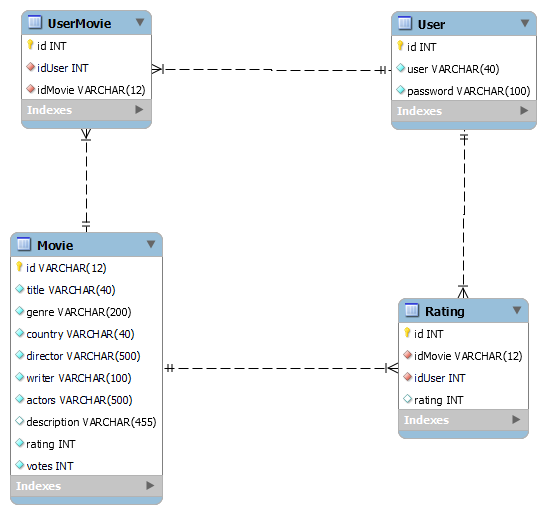
\includegraphics[width=10cm, height=10cm]{figures/diagrama db.png}}
\caption{Diagrama baza de date.}
\label{fig}
\end{figure}

\par Un lucru foarte important in dezvoltarea aplicatiei a fost alegerea bazei de date, am optat pentru pentru MySql versiunea 8.0. In tabelul de User voi salva datele de inregisrare a unui utilizator , in tabelul  Movie sunt prezente datele care descriu un film prin colloanele:title,genre,country,directors,writers,actors,description,votes si rating, in tabelul Rating salvez datele unui rating dat de un user pe laga valoare ratingului salvez si id-urile de la film si user pentru a stii cine da rating si la ce film totodata pe partea de back-end fac si o actualizare a rating ului si numarului de voturi din tabelul Movie asta pentru o a face aplicatia sa se miste mai rapid, iar in tabelul UserMovie salvez id ul de la un user si id ul de la un film reprezentand un film pe care utilizatorul l-a vizualizat.

\section{Server Node Js}
\label{sec:ch5sec1}

\par Serverul de Node Js il folosesc pentru a face inregistrare, login, returanrea tuturor filmelor care contin un numit sub titlu, adaugarea unui film la lista utilizatorului, returnarea a tuturor filmelor unui utilizator si adaugarea de rating a unui film. Cu ajutorul pachetului Express stabilesc rutele si pornesc serverul. Cand se face un request pe o ruta, se apeleaza functia asignata din Service, care are rol de a modela datele in functie de cum avem nevoie. Pentru a comunica cu baza de date ne folosim de Repository, acesta face legatura cu baza de date.

\subsection{Inregistrare}
\par Procesul de inregistrare este unul simplu, pasii fiind urmatorii:
\begin{enumerate}
  	\item Se trimit datele catre server
  	\item Se valideaza datele primite 
 	\item Daca datele sunt valide se verifica daca numele utilizatorului se afla in baza de date deoarece numele trebuie sa fie unic pentru fiecare utiliztor
	\item Daca totul este bine pana la acest pas se face has la parola pentru o mai buna securitate
		\begin{figure}[htbp]
			\centerline{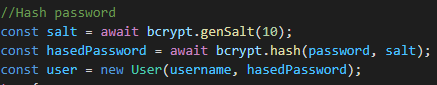
\includegraphics[width=15cm, height=4cm]{figures/hasparola.png}}
			\caption{Has la parola.}
			\label{fig}
		\end{figure}
	\item Următorul pas este de a apela functția din repositoy care adaugă un user in baza de date.
		\begin{figure}[htbp]
			\centerline{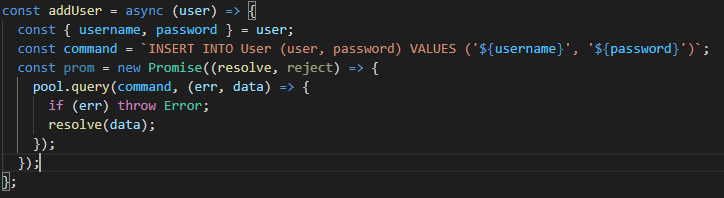
\includegraphics[width=19cm, height=6cm]{figures/adaugare user.png}}
			\caption{Adaugare user in baza de date.}
			\label{fig}
		\end{figure}	
	\item Dacă adăugarea s-a efectuat cu succes se returneaza un messaj de succes altfel se returnează un mesajul de eroare.
\end{enumerate}

\subsection{Autentificare}
\par Pașii pentru procesul de autentificare sunt următorii
\begin{enumerate}
  	\item Se trimit datele catre server
  	\item Se valideaza datele primite
  	\item Se verifica daca username-ul se afla in baza de date 
		\begin{figure}[htbp]
			\centerline{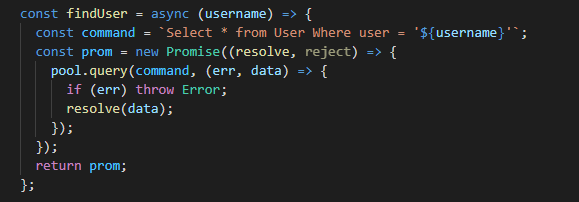
\includegraphics[width=19cm, height=6cm]{figures/cautare user.png}}
			\caption{Cautare dupa username in baza de date}
			\label{fig}
		\end{figure}	
	\item Daca se găsește user-ul in baza de date se verifică parola trimisă in requst cu cea din baza de date apoi se trimite raspunsul in functie de potrivirea celor doua parole, daca rapunsul este valid se va trimite id-ul user-ului care va reprezenta token-ul pentru front-end, daca  parolele nu corespund se va trimite status 400 si un mesaj de eroare.
		\begin{figure}[htbp]
			\centerline{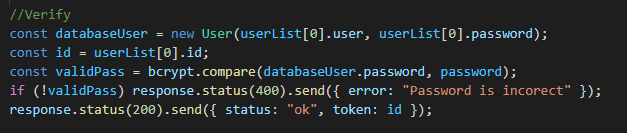
\includegraphics[width=19cm, height=6cm]{figures/verificare login.png}}
			\caption{Verificare parola si trimitere raspuns}
			\label{fig}
		\end{figure}	
\end{enumerate}
\chapter{Concluzii}
\section{Ce s-a obtinut}

\par Scopul aplicatiei a fost dezvoltarea unui algoritm care sa recomande filme si crearea unei aplicatii care sa ajute un utilizator sa isi poata nota toate filmele relevante pentru el, de exemplu filmele pe care el le-a vizualizat, totodata aceasta platforma sa recomande sa indrume utilizatorul spre alte filme facandu-i recomandari. Lucrarea si-a atins aceste scopuri puse la ineputul lucrari atat algoritmic cat si business. Obiectivul de business nu a fost unul principal mai mult necesar fiind pentru a putea interactiona cu algoritmul de recomandari.

\section{Ce s-a obtinut}
\par Un prim lucru ar fi experienta utilizatorului cu aplicatia dezvoltata, design-ul nu este cel mai reusit nefiin luati in calcul oameni cu dizabilitati nepunanduse accent pe utilizabilitatea interfetei.Tot odata aplicatia ar putea fi dezvoltata pentru a permite utilizatorului sa isi gestioneze mai bine filmele.
\par Pe partea de algoritm, acesta functioneaza si de multe ori face recomandari foarte utile,dar sunt momente cad da si rateuri cauza putand fiind multitudinea de cuvinte pe care filmele le au. O mai buna prelucrare a datelor ar ajuta algoritmul sa fie mult mai efficient.



%\addcontentsline{toc}{chapter}{Concluzii}
%\addcontentsline{toc}{chapter}{Conclusions}

\bibliography{c}

\end{document}
